\section{연구 결과}

\subsection{자료 처리}

\subsubsection{SST를 히스토그램}

Python으로 코딩하여 SST Figure \ref{fig:hist}\와 같이 자료의 히스토그램을 그려 자료의 신뢰도를 확인하였다. 

\begin{figure}[htbp]
	\centerline{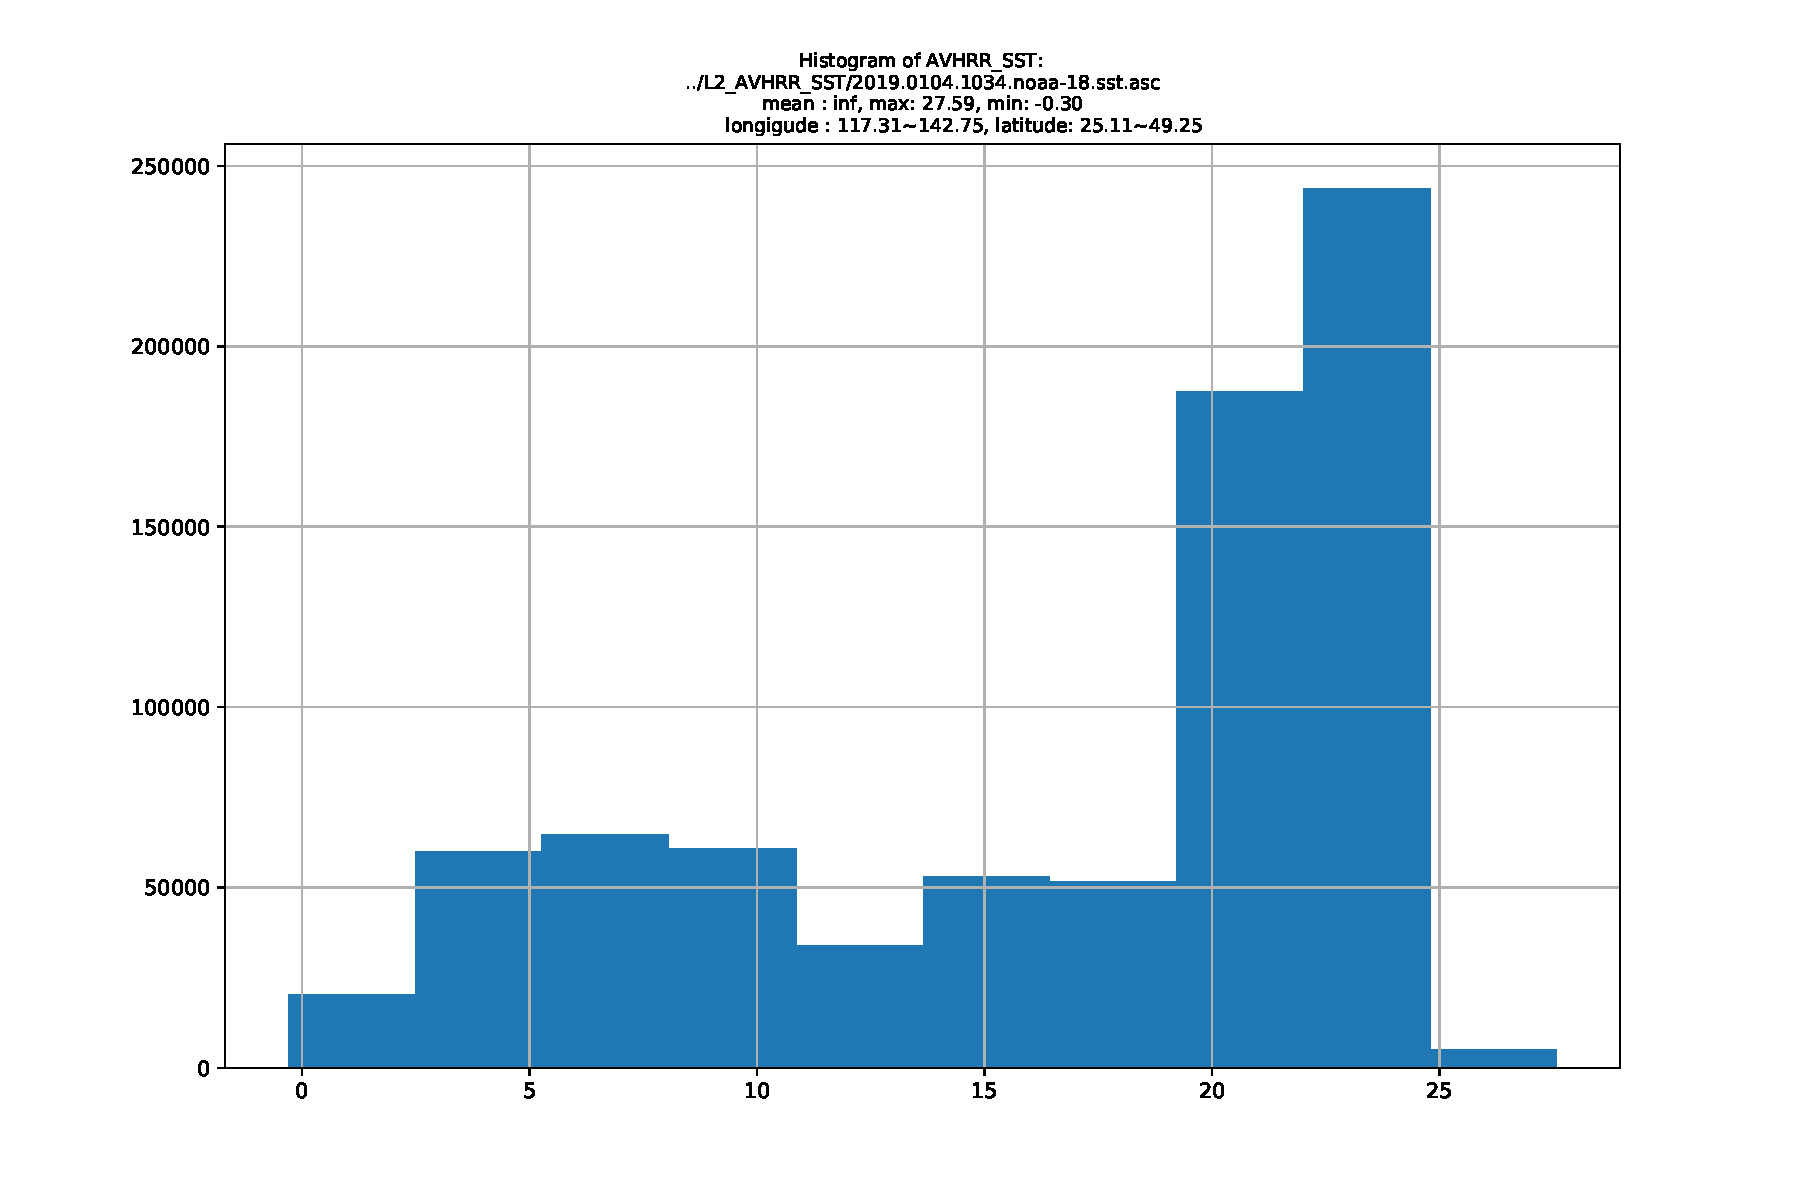
\includegraphics[trim=70 30 75 20, clip, width=\textwidth]{2019.0104.1034.noaa-18.sst_AVHRR_SST_hist}}
	\caption{SST의 히스토그램(NOAA/AVHRR).}
	\label{fig:hist}
\end{figure}

\newpage
\subsubsection{SST를 지도에 표출}

Python으로 코딩하여 SST 자료를 지도 위에 표출하였다. KOSC에서 배포한 자료와 색깔은 다르게 표출하였으나, 원하는 모양대로 자료를 표출할 수 있었다.

\begin{figure}[htbp]
	\begin{center}
		\begin{tabular}{cc}
			{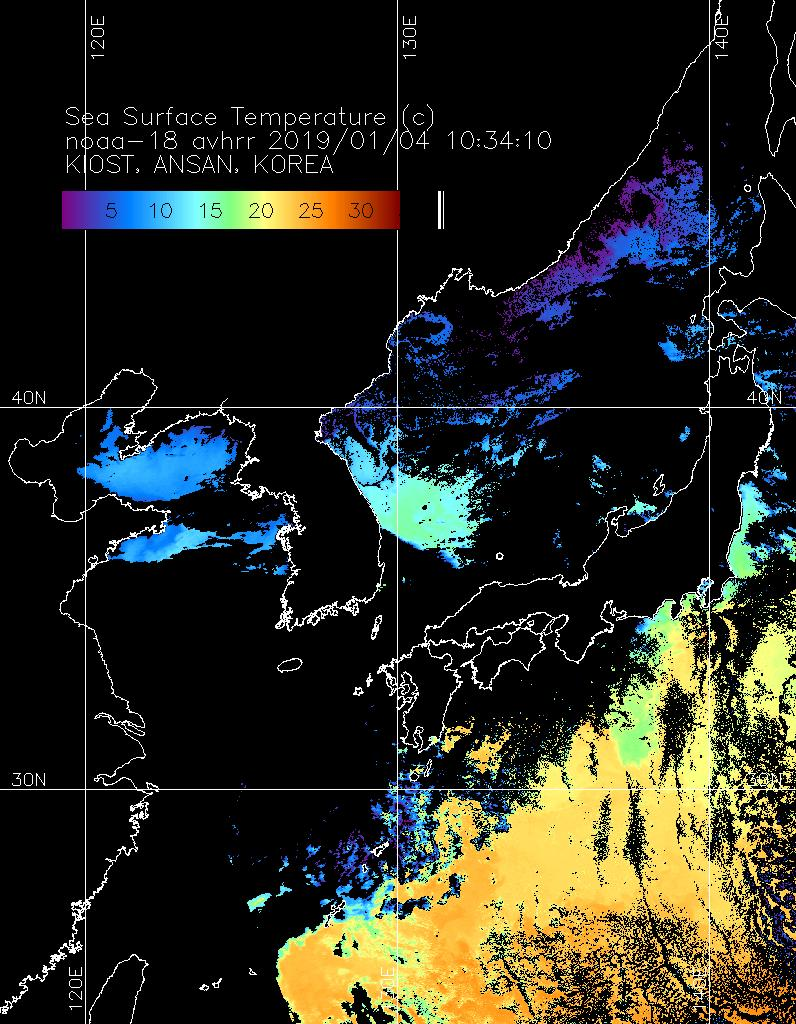
\includegraphics[width=6.2cm]{2019.0104.1034.noaa-18.sst}} &
			{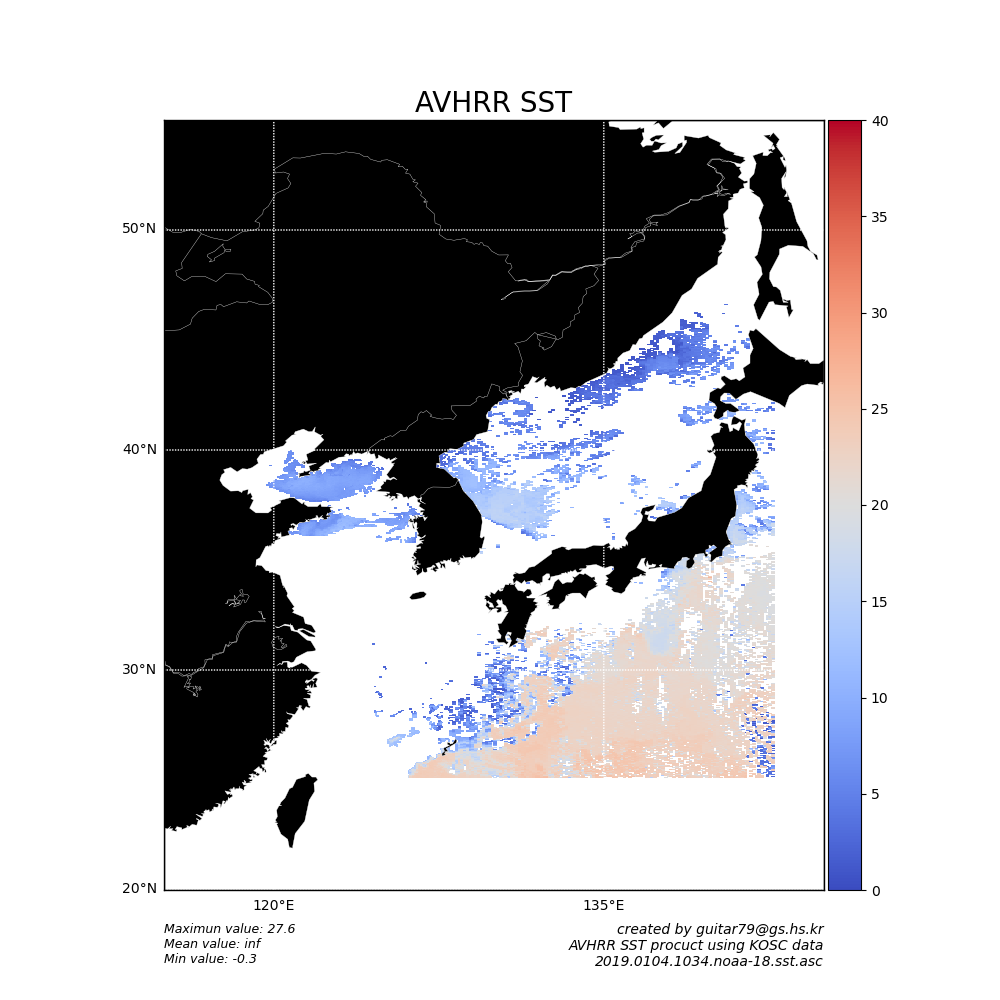
\includegraphics[trim=85 25 75 50, clip, width=7cm]{2019.0104.1034.noaa-18.sst_AVHRR_SST_map.png}}
		\end{tabular}
	\end{center}
	\begin{tikzpicture} [remember picture,overlay]
		\node[text=black] at (0.15, 8.4) {(a)};
		\node[text=black] at (7.15, 8.4) {(b)};
	\end{tikzpicture}	
	\caption{(a) KOSC에서 배포한 NOAA/AVHRR SST. (b) 직접 그린 NOAA/AVHRR SST.}	
	\label{fig:KOSC-self}
\end{figure}

\newpage
\subsection{레벨3 자료 산출}

\subsubsection{일평균값 산출}

일평균값의 레벨3 자료를 산출하여 Figure \ref{fig:daily_mean1}\과 같이 지도 위에 표출해 보았다. 

\begin{figure}[htbp]
	\centerline{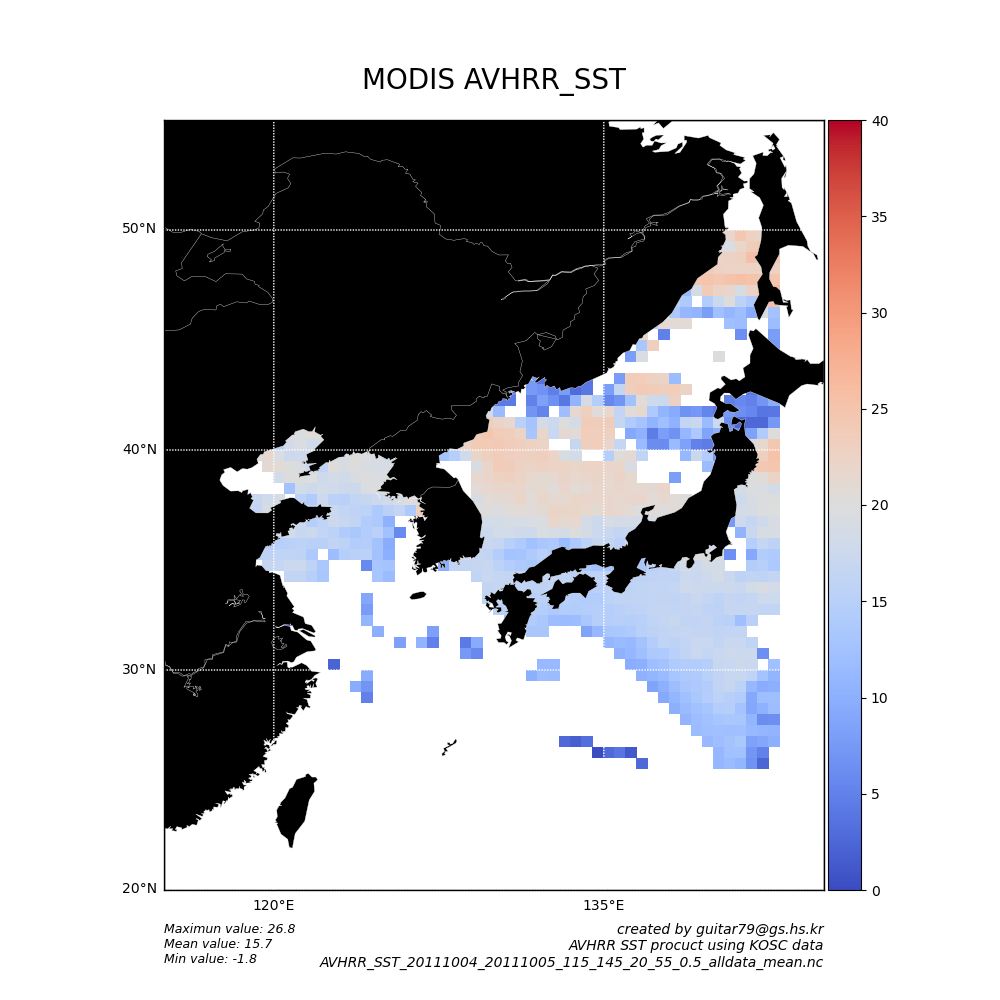
\includegraphics[width=\textwidth]{AVHRR_SST_20111004_20111005_115_145_20_55_0.5_alldata_mean_map.png}}
	\caption{SST 일평균값 산출 결과(NOAA/AVHRR).}
	\label{fig:daily_mean1}
\end{figure}

\newpage
\subsubsection{주평균값 산출}

주평균값의 레벨3 자료를 산출하여 Figure \ref{fig:weekly_mean1}\과 같이 지도 위에 표출해 보았다. 

\begin{figure}[htbp]
	\centerline{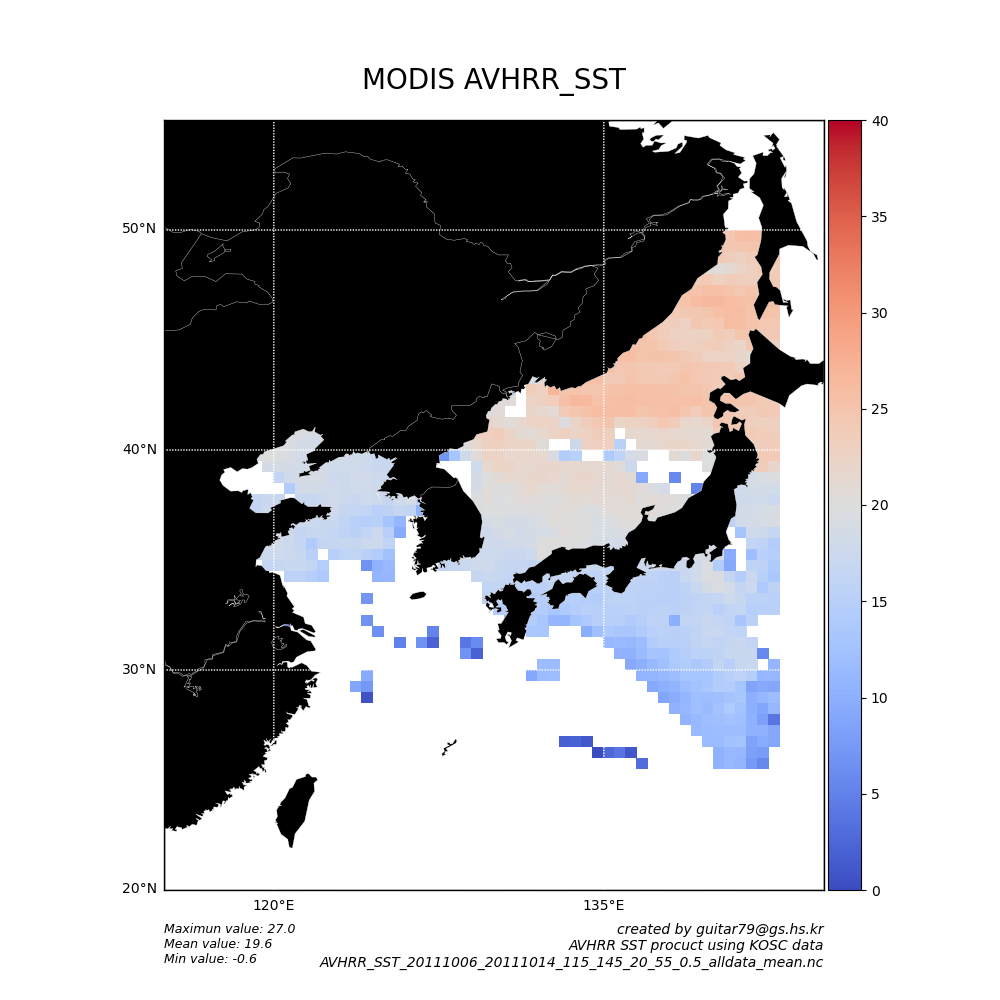
\includegraphics[width=\textwidth]{AVHRR_SST_20111006_20111014_115_145_20_55_0.5_alldata_mean_map.png}}
	\caption{SST 주평균값 산출 결과(NOAA/AVHRR).}
	\label{fig:weekly_mean1}
\end{figure}

\newpage
\subsubsection{월평균값 산출}

월평균값의 레벨3 자료를 산출하여 Figure \ref{fig:monthly_mean1}\과 같이 지도 위에 표출해 보았다. 

\begin{figure}[htbp]
	\centerline{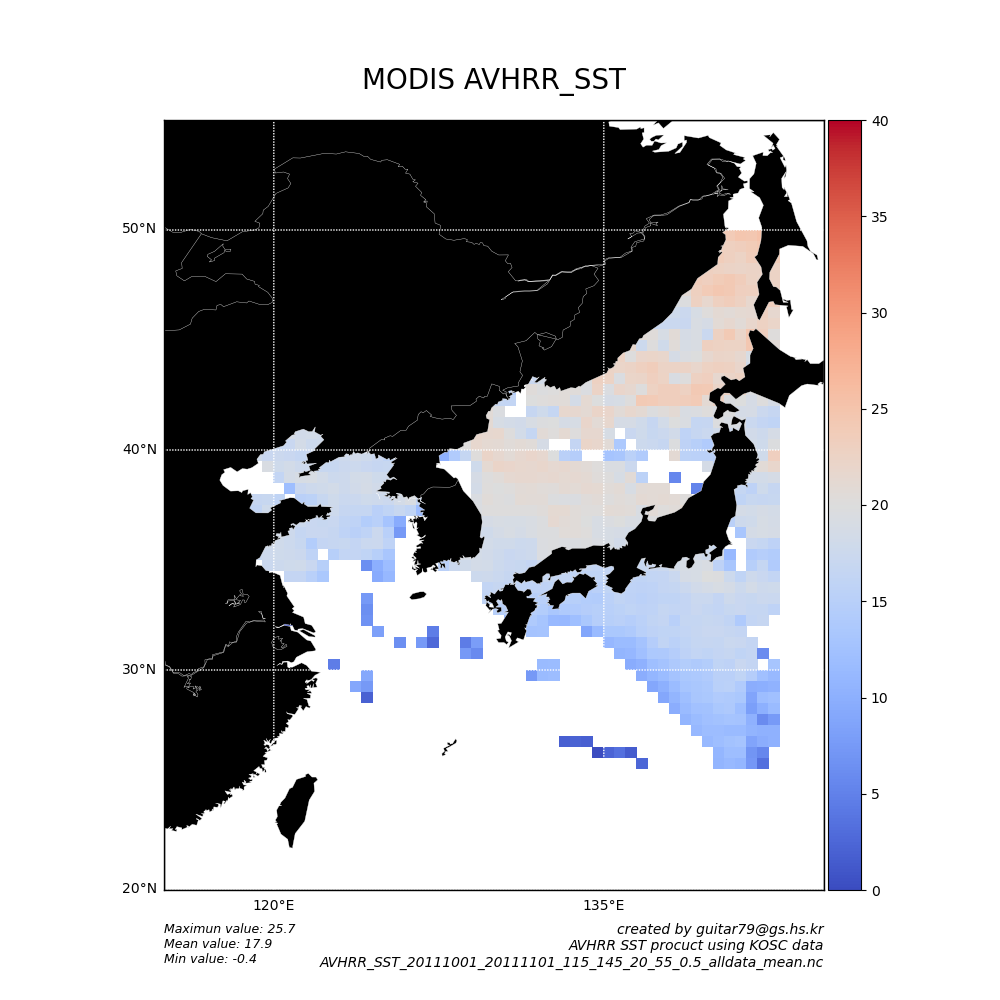
\includegraphics[width=\textwidth]{AVHRR_SST_20111001_20111101_115_145_20_55_0.5_alldata_mean_map.png}}
	\caption{SST 월평균값 산출 결과(NOAA/AVHRR).}
	\label{fig:monthly_mean1}
\end{figure}




